\chapter{Missingness Data}

\section{The Problem of Missing Data}

We concern the problem the analysis of such a data matrix when some of the entries in the matrix are not observed (Figure \ref{figure:examples-of-missingness-patterns}).

\begin{figure}[hpt]
	\centering
	\begin{subfigure}{.25\textwidth}
		\centering
		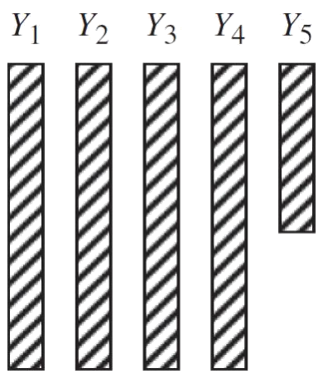
\includegraphics[width=\linewidth]{statistics-applications/figures/univariate-nonresponse.png}
		\caption{Univariate}
	\end{subfigure}
	\quad
	\begin{subfigure}{.25\textwidth}
		\centering
		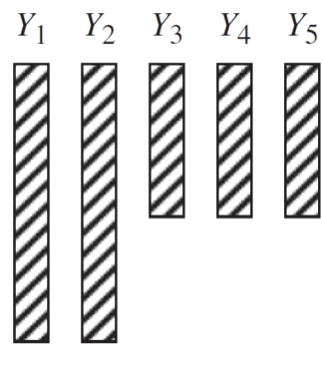
\includegraphics[width=\linewidth]{statistics-applications/figures/multivariate-nonresponse.png}
		\caption{Multivariate}
	\end{subfigure}
	\quad
	\begin{subfigure}{.25\textwidth}
		\centering
		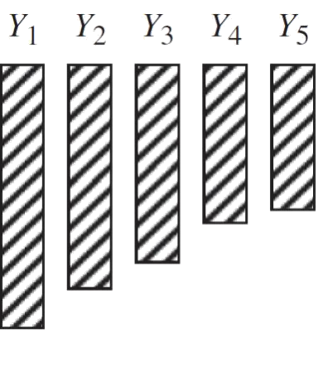
\includegraphics[width=\linewidth]{statistics-applications/figures/monotone-nonresponse.png}
		\caption{Monotone}
	\end{subfigure}
	\quad
	\begin{subfigure}{.25\textwidth}
		\centering
		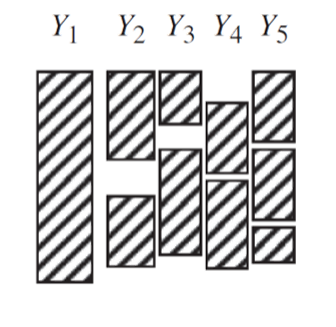
\includegraphics[width=\linewidth]{statistics-applications/figures/general-nonresponse.png}
		\caption{General}
	\end{subfigure}
	\quad
	\begin{subfigure}{.25\textwidth}
		\centering
		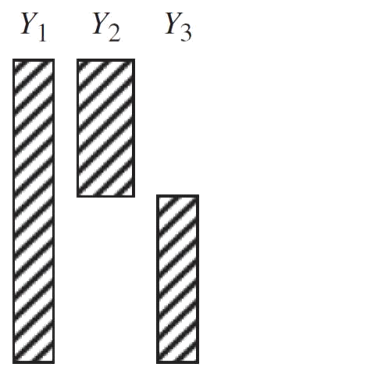
\includegraphics[width=\linewidth]{statistics-applications/figures/file-matching.png}
		\caption{File matching}
	\end{subfigure}
	\quad
	\begin{subfigure}{.25\textwidth}
		\centering
		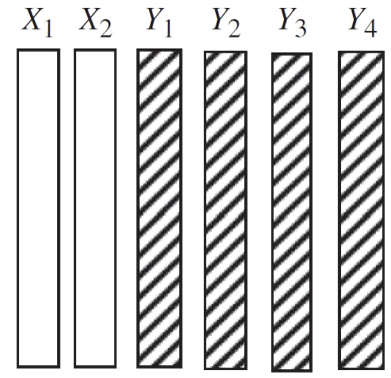
\includegraphics[width=\linewidth]{statistics-applications/figures/factor-analysis.png}
		\caption{Factor analysis}
	\end{subfigure}
	\caption{Examples of missingness patterns}
	\label{figure:examples-of-missingness-patterns}
\end{figure}

Notations for missing data are as follows
\begin{itemize}
	\item $Y=(y_{ij})$ denote the $(n\times p)$ rectangular data matrix, where only a portion of $Y$ are observed and $y_{ij}=\star$ indicates this entry is missing;
	\item $M=(m_{ij})$ denote the \textit{missingness indicator matrix} for $y_{ij}$, taking $m_{ij}=0$ for $y_{ij}$ is observed, and $m_{ij}=1$ for $y_{ij}$ is missing.
	\item In order to simplify, let $y_{i}=\left(y_{i1},y_{i2},\ldots,y_{ip}\right),\quad m_{i}=\left(m_{i1},m_{i2},\ldots,m_{ip}\right)$ and $y_{(0)i}$ be the components of $y_i$ that are observed for unit $i$, $y_{(1)i}$ be the components of $y_i$ that are missing for unit $i$.
\end{itemize}

\subsection{Missingness Mechanisms}

The missingness mechanism is characterized by the conditional distribution of $m_{i}$ given $y_{i}$, say
\begin{equation}
	f_{M\mid Y}\left(m_{i}\mid y_{i},\phi\right),
\end{equation}
where $\phi$ denotes unknown parameters.

\begin{definition}[Missing Completely at Random, MCAR]
	If missingness does not depend on the value of the data, missing or observed, i.e., if for all $y_{i}$ and any distinct values $y^{*}$ in the sample space of $Y$,
	\begin{equation}
		f_{M\mid Y}\left(m_{i} \mid y_{i},\phi\right)=f_{M\mid Y}\left(m_{i} \mid y^{*},\phi\right),
	\end{equation}
	then the data are called missing completely at random, MCAR.
\end{definition}

\begin{definition}[Missing at Random, MAR]
	If missingness depends on $y_{i}$ only through the observed components $y_{(0)}$, i.e., if for all $y_{i}$ and any distinct values $y_{(1)}^{*}$ in the sample space of $y_{(1)}$,
	\begin{equation}
		f_{M \mid Y}\left(m_{i}\mid y_{(0)i},y_{(1)i},\phi\right)=f_{M\mid Y}\left(m_{i}\mid y_{(0)i},y_{(1)}^{*},\phi\right),
	\end{equation}
	then the data are called missing at random, MAR.
\end{definition}

\begin{definition}[Missing Not at Random, MNAR]
	If missingness depends on $y_{i}$ the missing components $y_{(1)}$, i.e., if some $y_{i}$ and some values $y_{(1)}^{*}$ in the sample space of $y_{(1)}$,
	\begin{equation}
		f_{M \mid Y}\left(m_{i}\mid y_{(0)i},y_{(1)i},\phi\right)\neq f_{M\mid Y}\left(m_{i}\mid y_{(0)i},y_{(1)}^{*},\phi\right),
	\end{equation}
	then the data are called missing not at random, MNAR.
\end{definition}

\subsection{Commonly Used Methods for Missing Data}

\begin{enumerate}
	\item Complete-case Analysis: discard incompletely recorde units, only use the units with the complete data.
	\item Weighting Procedures: randomization inferences from sample survey data without nonresponse commonly weight sampled units by their design weights.
	\item Imputation Methods: impute the missing values, and the resultant completed data are analyzed by standard methods.
	\item \textbf{Model-based Methods}: A broad class of procedures is generated by defining a model for the complete data and basing inferences on the likelihood or posterior distribution under that model, with parameters estimated by procedures such as maximum likelihood.
	\item Hybrid Approaches: approaches based on estimating equations have been
	      proposed that combine the aspects of modeling and weighting.
\end{enumerate}

\section{Likelihood-Based Inference with Missing Data}

We can model the density of the joint distribution of $Y$ and $M$ using the "selection model" factorization
\begin{equation*}
	p(Y=y,M=m\mid\theta,\psi)=f_{Y}(y\mid\theta)f_{M\mid Y}(m\mid y,\psi),
\end{equation*}
where $\theta$ is the parameter vector governing the data model, and $\psi$ is the parameter vector governing the model for the missingness mechanism.

The full likelihood based on the observed values $\left(y_{(0)}, m\right)$ and the assumed joint distribution model above is defined to be
\begin{equation}
	L_{\text {full }}\left(\theta, \psi \mid y_{(0)}, m\right)=\int f_{Y}\left(y_{(0)}, y_{(1)} \mid \theta\right) f_{M \mid Y}\left(m \mid y_{(0)}, y_{(1)}, \psi\right) \mathrm{d} y_{(1)}
\end{equation}

The likelihood of $\theta$ ignoring the missingness mechanism is defined to be
\begin{equation}
	L_{\mathrm{ign}}\left(\theta \mid y_{(0)}\right)=\int f_{Y}\left(y_{(0)}, y_{(1)} \mid \theta\right) \mathrm{d} y_{(1)}
\end{equation}

\subsection{Ignorable Missingness Mechanism}

\begin{definition}[Ignorable missingness mechanism]
	The missingness mechanism is called ignorable if for any given $\tilde{m}$ and  $\tilde{y}_{(0)}$ the inferences for $\theta$ based on the ignorable likelihood equation evaluated at $m=\tilde{m}$ and $\tilde{y}_{0}$ are the same as the full likelihood equation.
\end{definition}

\begin{remark}[Another definition of ignorable missingness mechanism]
	\begin{equation}
		\frac{L_{\text {full }}\left(\theta, \psi \mid \tilde{y}_{(0)}, \tilde{m}\right)}{L_{\text {full }}\left(\theta^{*}, \psi \mid \tilde{y}_{(0)}, \tilde{m}\right)}=\frac{L_{\text {ign }}\left(\theta \mid \tilde{y}_{(0)}\right)}{L_{\text {ign }}\left(\theta^{*} \mid \tilde{y}_{(0)}\right)} \quad \forall \theta, \theta^{*}, \psi .
	\end{equation}
\end{remark}

\begin{theorem}
	The missingness mechanism is ignorable for direct likelihood inference on $\left(\tilde{m},\tilde{y}_{(0)}\right)$ if
	\begin{enumerate}
		\item Parameter distinctness: The parameters $\theta$ and $\psi$ are distinct, that is, $\Omega_{\theta, \psi}=\Omega_{\theta} \times \Omega_{\psi}$.
		\item Factorization of the full likelihood: The full likelihood, with $\left(y_{0}, m\right)=\left(\tilde{y}_{0}, \tilde{m}\right)$ factors as
		      \begin{equation}
			      L_{\text{full}}\left(\theta,\psi\mid\tilde{y}_{(0)},\tilde{m}\right)=L_{\text{ign}}\left(\theta\mid\tilde{y}_{(0)}\right)\times L_{\text{rest}}\left(\psi\mid\tilde{y}_{(0)},\tilde{m}\right)\quad\forall\theta,\psi\in\Omega_{\theta,\psi}
			      \label{equation:factorization-of-the-full-likelihood}
		      \end{equation}
	\end{enumerate}
\end{theorem}

\begin{corollary}
	If the missing data are MAR at $\left(\tilde{m}, \tilde{y}_{(0)}\right)$, and $\theta$ and $\psi$ are distinct, the missingness mechanism is ignorable for likelihood inference.
\end{corollary}

\begin{proof}
	Since,
	\begin{equation}
		f_{M \mid Y}\left(\tilde{m} \mid \tilde{y}_{(0)}, y_{(1)}, \psi\right)=f_{M \mid Y}\left(\tilde{m} \mid \tilde{y}_{(0)}, y_{(1)}^{*}, \psi\right) \quad \forall y_{(1)}, y_{(1)}^{*}, \psi
	\end{equation}
	therefore,
	\begin{equation}
		\begin{aligned}
			  & f\left(\tilde{y}_{(0)}, \tilde{m} \mid \theta, \psi\right)=f_{M \mid Y}\left(\tilde{m} \mid \tilde{y}_{(0)}, \psi\right) \times \int f_{Y}\left(\tilde{y}_{(0)}, y_{(1)} \mid \theta\right) \mathrm{d} y_{(1)} \\
			= & f_{M \mid Y}\left(\tilde{m} \mid \tilde{y}_{(0)}, \psi\right) \times f_{Y}\left(\tilde{y}_{(0)} \mid \theta\right)
		\end{aligned}
	\end{equation}
	yields the factored likelihood equation \ref{equation:factorization-of-the-full-likelihood}.
\end{proof}

\subsubsection{Ignorable Missingness Mechanism v.s. Nonignorable Missingness Mechanism}

\begin{example}[Exponential Sample]
	The joint density of $n$ independent and identically distributed scalar units from the exponential distribution with mean $\theta>0$ is
	\begin{equation}
		f_{Y}(y\mid\theta)=\theta^{-n}\exp\left\{-\sum_{i=1}^{n}\frac{y_{i}}{\theta}\right\}.
	\end{equation}

	The loglikelihood fuction is
	\begin{equation}
		\ell_{Y}(\theta\mid y)=\ln\left\{\theta^{-n}\exp\left(-\sum_{i=1}^{n}\frac{y_{i}}{\theta}\right)\right\}=-n\ln\theta-\sum_{i=1}^{n}\frac{y_{i}}{\theta}.
	\end{equation}

	Differentiating with respect to $\theta$ gives the likelihood equation
	\begin{equation}
		-\frac{n}{\theta}+\sum_{i=1}^{n} \frac{y_{i}}{\theta^{2}}=0.
	\end{equation}

	Thus, we obtain the ML estimates
	\begin{equation}
		\hat{\theta}=\bar{y}=\frac{1}{n}\sum_{i=1}^{n}y_i.
	\end{equation}
\end{example}

\begin{example}[Incomplete Exponential Sample]
	Suppose we have an incomplete univariate exponential sample with $y_{(0)}=\left(y_{1},\ldots,y_{r}\right)^{\mathrm{T}}$ observed and $y_{(1)}=\left(y_{r+1},\ldots,y_{n}\right)^{\mathrm{T}}$ missing. Thus, $m=\left(m_{1},\ldots,m_{n}\right)^{\mathrm{T}}$, where $m_{i}=0,i=1,\ldots,r$ and $m_{i}=1,i=r+1,\ldots,n$.

	The likelihood ignoring the missingness mechanism is
	\begin{equation}
		L_{\mathrm{ign}}\left(\theta\mid y_{(0)}\right)=\theta^{-r}\exp\left(-\sum_{i=1}^{r}\frac{y_{i}}{\theta}\right).
	\end{equation}

	If each unit is observed with probability $\psi$ that does not depend on $Y$, that is,
	\begin{equation}
		f_{M\mid Y}(m\mid y,\psi)=\frac{n!}{r!(n-r)!}\psi^{r}(1-\psi)^{n-r}
	\end{equation}
	then,
	\begin{equation}
		f\left(y_{(0)},m\mid\theta,\psi\right)=\frac{n!}{r!(n-r)!}\psi^{r}(1-\psi)^{n-r}\theta^{-r}\exp\left(-\sum_{i=1}^{r}\frac{y_{i}}{\theta}\right)
	\end{equation}
	Because the missing data are MAR, if $\psi$ and $\theta$ are distinct, then likelihood-based
	inferences about $\theta$ can be based on the ignorable likelihood, the ML estimate of $\theta$ is
	\begin{equation}
		\hat{\theta}=\frac{1}{r}\sum_{i=1}^{r}y_{i}.
	\end{equation}

	If each unit is observed only if values less than $c$, that is
	\begin{equation}
		f_{M\mid Y}(m\mid y,\psi)=\prod_{i=1}^{n}f\left(m_{i}\mid y_{i},\psi\right),
	\end{equation}
	where
	\begin{equation}
		f\left(m_{i} \mid y_{i}, \psi\right)=\left\{\begin{array}{ll}
			1, & y_{i}\geq c        \\
			0, & \text{ otherwise }
		\end{array}\right.
	\end{equation}
	Hence,
	\begin{equation}
		\begin{aligned}
			L_{\text {full }}\left(\theta \mid y_{(0)}, m\right) & =\prod_{i=1}^{r} f_{Y}\left(y_{i} \mid \theta\right) \operatorname{Pr}\left(y_{i}<c \mid y_{i}, \theta\right) \times \prod_{i=r+1}^{n} \operatorname{Pr}\left(y_{i} \geq c \mid \theta\right) \\
			                                                     & =\theta^{-r} \exp \left(-\sum_{1}^{r} \frac{y_{i}}{\theta}\right) \times \exp \left(-\frac{(n-r) c}{\theta}\right)
		\end{aligned}
	\end{equation}
	Maximizing above equation with respect to $\theta$ gives the ML estimate
	\begin{equation}
		\hat{\theta}=\frac{1}{r}\left[\sum_{i=1}^{r}y_{i}+(n-r)c\right].
	\end{equation}

	The inflation of the sample mean in this expression reflects the censoring of the missing values.
\end{example}

\subsection{Expectation-Maximization Algorithm}

Let $\theta^{(i)}$ be the current estimate of the parameter $\theta .$ The E step of EM finds the expected complete-data loglikelihood if $\theta$ were $\theta^{(t)}$:
\begin{equation}
	Q\left(\theta \mid \theta^{(t)}\right)=\int\ell\left(\theta \mid Y_{(0)}, Y_{(1)}\right) f\left(Y_{(1)} \mid Y_{(0)}, \theta^{(t)}\right) \mathrm{d} Y_{(1)}.
\end{equation}

The M step of EM determines $\theta^{(t+1)}$ by maximizing this expected completedata loglikelihood:
\begin{equation}
	Q\left(\theta^{(t+1)} \mid \theta^{(t)}\right) \geq Q\left(\theta \mid \theta^{(t)}\right), \quad \forall\theta.
\end{equation}

Hence, EM algorithm for likelihood-based inference with missing data is
\begin{enumerate}
	\item replace missing values by estimated
	      values
	\item estimate parameters
	\item re-estimate the missing values assuming the new parameter estimates are correct
	\item re-estimate parameters, and so forth, iterating until apparent convergence
\end{enumerate}

\subsubsection{Convergence Properties of EM Algorithm with Missing Data}

\begin{theorem}
	Every GEM algorithm increases $\ell\left(\theta \mid Y_{(0)}\right)$ at each iteration, that is,
	\begin{equation}
		\ell\left(\theta^{(t+1)} \mid Y_{(0)}\right) \geq \ell\left(\theta^{(t)} \mid Y_{(0)}\right)
	\end{equation}
	, with equality if and only if
	\begin{equation}
		Q\left(\theta^{(t+1)} \mid \theta^{(t)}\right)=Q\left(\theta^{(t)} \mid \theta^{(t)}\right)
	\end{equation}
\end{theorem}

\begin{proof}
	The distribution of the complete data Y can be factored as follows:
	\begin{equation}
		f(Y \mid \theta)=f\left(Y_{(0)}, Y_{(1)} \mid \theta\right)=f\left(Y_{(0)} \mid \theta\right) f\left(Y_{(1)} \mid Y_{(0)}, \theta\right)
	\end{equation}

	The corresponding decomposition of the loglikelihood is
	\begin{equation}
		\ell(\theta \mid Y)=\ell\left(\theta \mid Y_{(0)}, Y_{(1)}\right)=\ell\left(\theta \mid Y_{(0)}\right)+\ln f\left(Y_{(1)} \mid Y_{(0)}, \theta\right)
	\end{equation}

	Let,
	\begin{equation}
		\ell\left(\theta \mid Y_{(0)}\right)=\ell(\theta \mid Y)-\ln f\left(Y_{(1)} \mid Y_{(0)}, \theta\right)
	\end{equation}

	The expectation of both sides of above equation over the distribution of the missing data $Y_{(1)}$, given the observed data $Y_{(0)}$ and a current estimate of $\theta$, say $\theta_{(t)}$, is
	\begin{equation}
		\ell\left(\theta \mid Y_{(0)}\right)=Q\left(\theta \mid \theta^{(t)}\right)-H\left(\theta \mid \theta^{(t)}\right)
	\end{equation}
	, where
	\begin{equation}
		\begin{aligned}
			Q\left(\theta \mid \theta^{(t)}\right)= & \int\ell\left(\theta \mid Y_{(0)}, Y_{(1)}\right) f\left(Y_{(1)} \mid Y_{(0)}, \theta^{(t)}\right) \mathrm{d} Y_{(1)} \\
			H\left(\theta\mid\theta^{(t)}\right)=   & \int\ln f\left(Y_{(1)}\mid Y_{(0)},\theta\right)f\left(Y_{(1)} \mid Y_{(0)}, \theta^{(t)}\right) \mathrm{d} Y_{(1)}
		\end{aligned}
	\end{equation}

	Since,
	\begin{equation}
		\begin{aligned}
			     & H\left(\theta^{(t)},\theta^{(t)}\right)-H\left(\theta,\theta^{(t)}\right)                                                                                                           \\
			=    & \int\ln f\left(Y_{(1)}\mid Y_{(0)},\theta^{(t)}\right)f\left(Y_{(1)}\mid Y_{(0)},\theta^{(t)}\right)\mathrm{d}Y_{(1)}                                                               \\
			     & -\int\ln f\left(Y_{(1)}\mid Y_{(0)},\theta\right))f\left(Y_{(1)}\mid Y_{(0)},\theta^{(t)}\right)\mathrm{d}Y_{(1)}                                                                   \\
			=    & \int\ln\left[\frac{f\left(Y_{(1)}\mid Y_{(0)},\theta^{(t)}\right)}{f\left(Y_{(1)}\mid Y_{(0)},\theta\right)}\right]f\left(Y_{(1)}\mid Y_{(0)},\theta^{(t)}\right)\mathrm{d}Y_{(1)}  \\
			=    & \int-\ln\left[\frac{f\left(Y_{(1)}\mid Y_{(0)},\theta\right)}{f\left(Y_{(1)}\mid Y_{(0)},\theta^{(t)}\right)}\right]f\left(Y_{(1)}\mid Y_{(0)},\theta^{(t)}\right)\mathrm{d}Y_{(1)} \\
			\geq & -\ln\int\frac{f\left(Y_{(1)}\mid Y_{(0)},\theta\right)}{f\left(Y_{(1)}\mid Y_{(0)},\theta^{(t)}\right)}f\left(Y_{(1)}\mid Y_{(0)},\theta^{(t)}\right)\mathrm{d}Y_{(1)}=0
		\end{aligned}
	\end{equation}

	Therefore,
	\begin{equation}
		H\left(\theta \mid \theta^{(t)}\right) \leq H\left(\theta^{(t)} \mid \theta^{(t)}\right)
	\end{equation}

	Hence, the difference in values of $\ell\left(\theta \mid Y_{(0)}\right)$ at successive iterates is given by
	\begin{equation}
		\begin{aligned}
			\ell\left(\theta^{(t+1)} \mid Y_{(0)}\right)-\ell\left(\theta^{(t)} \mid Y_{(0)}\right)= & \left[Q\left(\theta^{(t+1)} \mid \theta^{(t)}\right)-Q\left(\theta^{(t)} \mid \theta^{(t)}\right)\right]  \\
			                                                                                         & -\left[H\left(\theta^{(t+1)} \mid \theta^{(t)}\right)-H\left(\theta^{(t)} \mid \theta^{(t)}\right)\right] \\
			\geq                                                                                     & 0
		\end{aligned}
	\end{equation}
\end{proof}

\begin{theorem}
	Suppose a sequence of EM iterates is such that
	\begin{enumerate}
		\item $D^{10} Q\left(\theta^{(t+1)} \mid \theta^{(t)}\right)=0$, where "D" here denotes derivative, and $D^{10}$ means the derivative with respect to the first argument, that is, define
		      \begin{equation}
			      D^{10} Q\left(\theta^{(t+1)}\mid\theta^{(t)}\right)=\left.\frac{\partial}{\partial \theta} Q\left(\theta \mid \theta^{(t)}\right)\right|_{\theta=\theta^{(t+1)}}=0.
		      \end{equation}
		\item $\theta^{(t)}$ converges to $\theta^{*}$.
		\item $f\left(Y_{(1)} \mid Y_{(0)}, \theta\right)$ is smooth in $\theta$, where smooth is defined in the proof.
	\end{enumerate}
	Then
	\begin{equation}
		\left.D \ell\left(\theta^{*} \mid Y_{(0)}\right) \equiv \frac{\partial}{\partial \theta} \ell\left(\theta \mid Y_{(0)}\right)\right|_{\theta=\theta^{*}}=0,
	\end{equation}
	so that if the $\theta^{(t)}$ converge, they converge to a stationary point.
\end{theorem}

\begin{proof}
	\begin{equation}
		\begin{aligned}
			D \ell\left(\theta^{(t+1)} \mid Y_{(0)}\right) & =D^{10} Q\left(\theta^{(t+1)} \mid \theta^{(t)}\right)-D^{10} H\left(\theta^{(t+1)} \mid \theta^{(t)}\right)                                                                                       \\
			                                               & =-D^{10} H\left(\theta^{(t+1)} \mid \theta^{(t)}\right)                                                                                                                                            \\
			                                               & =-\left.\frac{\partial}{\partial \theta} \int\left[\ln f\left(Y_{(1)} \mid Y_{(0)}, \theta\right)\right] f\left(Y_{(1)} \mid Y_{(0)}, \theta^{(t)}\right) d Y_{(1)}\right|_{\theta=\theta^{(t+1)}}
		\end{aligned}
	\end{equation}
	which assuming sufficient smoothness to interchange the order of differentiation and integration,
	\begin{equation}
		\begin{aligned}
			= & -\int\left.\frac{\partial}{\partial \theta} f\left(Y_{(1)} \mid Y_{(0)}, \theta\right) d Y_{(1)}\right|_{\theta=\theta^{(t+1)}}    \\
			= & -\left.\int \frac{\partial}{\partial \theta} f\left(Y_{(1)} \mid Y_{(0)}, \theta\right) d Y_{(1)}\right|_{\theta=\theta^{(t+1)}}=0
		\end{aligned}
	\end{equation}
\end{proof}

\subsubsection{Examples of EM Algorithm with Missing Data}

\begin{example}[Multivariate Normal Sample]
	Let $y=\left(y_{i j}\right)$, where $i=1, \ldots, n$, $j=1, \ldots, p$, be a matrix representing an independent and identically distributed sample of $n$ units from the multivariate normal distribution with mean vector $\mu=\left(\mu_{1}, \ldots, \mu_{p}\right)$ and covariance matrix $\Sigma=(\sigma_{j k})$, $j=1, \ldots, p$; $k=1,\ldots, p$. Thus, $y_{i j}$ represents the value of the jth variable for the ith unit in the sample. The density of $y$ is
	\begin{equation}
		f_{Y}(y\mid\mu,\Sigma)=(2 \pi)^{-n p / 2}|\Sigma|^{-n / 2} \exp \left\{-\frac{1}{2} \sum_{i=1}^{n}\left(y_{i}-\mu\right) \Sigma^{-1}\left(y_{i}-\mu\right)^{\mathrm{T}}\right\}.
	\end{equation}

	The loglikelihood of $\theta=(\mu, \Sigma)$ is then
	\begin{equation}
		\ell_{Y}(\mu, \Sigma \mid y)=-\frac{n}{2}\ln |\Sigma|-\frac{1}{2} \sum_{i=1}^{n}\left(y_{i}-\mu\right) \Sigma^{-1}\left(y_{i}-\mu\right)^{\mathrm{T}}
	\end{equation}

	Maximizing above equation with respect to $\theta$ and $\Sigma$ gives the ML estimate
	\begin{equation}
		\hat{\mu}=\bar{y},\quad \hat{\Sigma}=\frac{n-1}{n}S,
	\end{equation}
	where $\bar{y}=\left(\bar{y}_{1}, \ldots, \bar{y}_{p}\right)$ is the row vector of sample means, and $S=\left(s_{j k}\right)$ is the $(p\times p)$ sample covariance matrix with $(j, k)$ th element $s_{j k}=\frac{1}{n-1}\sum_{i=1}^{n}\left(y_{i j}-\bar{y}_{i}\right)\left(y_{i k}-\bar{y}_{k}\right)$
\end{example}

\begin{example}[Incomplete Multivariate Normal Sample]
	Suppose $Y=\left(Y_{(0)}, Y_{(1)}\right)$, where $Y$ represents a random sample of size $n$ on $\left(Y_{1}, \ldots, Y_{p}\right), Y_{(0)}$ the set of observed values, and $Y_{(1)}$ the missing data. Also, let $y_{(0), i}$ represent the set of variables with values observed for unit $i, \quad i=1, \ldots, n$.

	The loglikelihood based on the observed data is then
	\begin{equation}
		\ell\left(\mu, \Sigma \mid Y_{(0)}\right)=-\frac{1}{2} \sum_{i=1}^{n} \ln \left|\Sigma_{(0), i}\right|-\frac{1}{2} \sum_{i=1}^{n}\left(y_{(0), i}-\mu_{(0), i}\right)^{\mathrm{T}} \Sigma_{(0), i}^{-1}\left(y_{(0), i}-\mu_{(0), i}\right)
	\end{equation}
	, where $\mu_{(0), i}$ and $\Sigma_{(0), i}$ are the mean and covariance matrix of the observed components of $Y$ for unit $i$.

	The exponential family form of multivariate normal distribution with $\left(\mu,\Sigma\right)$ is
	\begin{equation}
		f_{Y}(y\mid\mu,\Sigma)=(2\pi)^{-np/2}|\Lambda|^{n/2}\exp\left[\eta^{T}\sum_{i=1}^{n}y_{i}-\frac{1}{2}\sum_{i=1}^{n}\operatorname{tr}\left(\Lambda y_{i}y_{i}^{T}\right)-\frac{n}{2}\eta^{T}\Lambda\eta\right]
	\end{equation}
	, where $\Lambda=\Sigma^{-1}$ and $\eta=\Sigma^{-1}\mu$. And
	\begin{equation}
		\ln f_{Y}(y\mid\mu,\Sigma)=-\frac{np}{2}\ln(2\pi)+\frac{n}{2}\ln|\Lambda|-\frac{n}{2}\eta^{T}\Lambda\eta+\eta^{T}\sum_{i=1}^{n}y_{i}-\frac{1}{2}\sum_{i=1}^{n}\operatorname{tr}\left(\Lambda y_{i}y_{i}^{T}\right)
	\end{equation}

	Hence,
	\begin{equation}
		\begin{aligned}
			  & Q\left(\theta\mid\theta^{(t)}\right)=E_{Y_{(0)},\theta^{(t)}}\left[\ell\left(\theta\mid Y_{(0)},Y_{(1)}\right)\right]                  \\
			= & -\frac{np}{2}\ln(2\pi)+\frac{n}{2}\ln|\Lambda|-\frac{n}{2}\eta^{T}\Lambda\eta                                                          \\
			  & +\eta^{T}E\left(\sum_{i=1}^{n}y_{i}\right)-\frac{1}{2}\sum_{i=1}^{n}\operatorname{tr}\left(\Lambda E\left(y_{i}y_{i}^{T}\right)\right)
		\end{aligned}
	\end{equation}

	Therefore, the EM algorithm for incomplete multivariate normal sample is,
	\begin{itemize}
		\item E-step:
		      \begin{equation}
			      \begin{aligned}
				      E\left(\sum_{i=1}^{n} y_{i j} \mid Y_{(0)}, \theta^{(t)}\right)=         & \sum_{i=1}^{n} y_{i j}^{(t+1)}, \quad j=1, \ldots, p                                                  \\
				      E\left(\sum_{i=1}^{n} y_{i j} y_{i k} \mid Y_{(0)}, \theta^{(t)}\right)= & \sum_{i=1}^{n}\left(y_{i j}^{(t+1)} y_{i k}^{(t+1)}+c_{j k i}^{(t+1)}\right), \quad j, k=1, \ldots, p
			      \end{aligned}
		      \end{equation}
		      where
		      \begin{equation}
			      \begin{aligned}
				      y_{i j}^{(t+1)}=   & \left\{\begin{array}{ll}
					                                  y_{i j},                                             & \text { if } y_{i j} \text { is observed} \\
					                                  E\left(y_{i j} \mid y_{(0), i}, \theta^{(t)}\right), & \text { if } y_{i j} \text { is missing}
				                                  \end{array}\right.                                                                          \\
				      c_{j k i}^{(t+1)}= & \left\{\begin{array}{ll}
					                                  0,                                                                             & \text { if } y_{i j} \text { or } y_{i k} \text { is observed}  \\
					                                  \operatorname{Cov}\left(y_{i j}, y_{i k} \mid y_{(0), i}, \theta^{(t)}\right), & \text { if } y_{i j} \text { and } y_{i k} \text { are missing}
				                                  \end{array}\right.
			      \end{aligned}
		      \end{equation}

		\item M-step:
		      \begin{equation}
			      \begin{aligned}
				      \mu_{j}^{(t+1)}      & =n^{-1} \sum_{i=1}^{n} y_{i j}^{(t+1)}, \quad j=1, \ldots, p                                                                                                           \\
				      \sigma_{j k}^{(t+1)} & =n^{-1} E\left(\sum_{i=1}^{n} y_{i j} y_{i k} \mid Y_{(0)}, \theta^{(t)}\right)-\mu_{j}^{(t+1)} \mu_{k}^{(t+1)}                                                        \\
				                           & =n^{-1} \sum_{i=1}^{n}\left[\left(y_{i j}^{(t+1)}-\mu_{j}^{(t+1)}\right)\left(y_{i k}^{(t+1)}-\mu_{k}^{(t+1)}\right)+c_{j k i}^{(t+1)}\right], \quad j, k=1, \ldots, p
			      \end{aligned}
		      \end{equation}
	\end{itemize}
\end{example}

\begin{example}[Missing Outcomes in Multiple Linear Regression]
	Suppose a scalar outcome variable $Y$ is regressed on $p$ predictor variables $X_{1},\ldots,X_{p}$, $y_{i},i=1,\ldots,m$ are missing, where
	\begin{equation}
		\begin{aligned}
			E\left(Y \mid X_{1}, \ldots, X_{p}\right)                  & =\beta_{0}+\sum_{j=1}^{p} \beta_{j} X_{j} \\
			\operatorname{Var}\left(Y \mid X_{1}, \ldots, X_{p}\right) & =\sigma^{2}
		\end{aligned}
	\end{equation}

	We assume the joint distribution of the data (including outcomes and predictors) is multivariate normal with
	\begin{equation}
		\begin{aligned}
			\mu    & =\left(\mu_{1}, \ldots, \mu_{p}, \mu_{y}\right) \\
			\Sigma & =\left(\begin{array}{ll}
				                \Sigma_{x x} & \Sigma_{x y} \\
				                \Sigma_{y x} & \sigma_{y y}
			                \end{array}\right)
		\end{aligned}
	\end{equation}
	, and that the missing data mechanism is ignorable.

	Standard regression theory gives
	\begin{equation}
		\begin{array}{c}
			\beta=\boldsymbol{\Sigma}_{y x} \boldsymbol{\Sigma}_{x x}^{-1} ; \quad \beta_{0}=\mu_{y}-\sum_{j=1}^{p} \beta_{j} \mu_{j} ; \\
			\sigma^{2}=\sigma_{y y}-\boldsymbol{\Sigma}_{y x} \boldsymbol{\Sigma}_{x x}^{-1} \boldsymbol{\Sigma}_{x y}
		\end{array}
	\end{equation}

	The loglikelihood based on the observed data of $\theta=\left(\beta,\sigma^{2}\right)$, where $\beta=\left(\beta_{0},\beta_{1},\ldots,\beta_{p}\right)$, given observed data $\left\{\left(x_{i},y_{i}\right),i=1,\ldots,n\right\}$ is
	\begin{equation}
		\ell(\beta, \sigma^{2} \mid X, Y_{(0)})=-\frac{n-m}{2}\ln\sigma^2-\frac{1}{2}\sum_{i=m+1}^{n}\left(y_{i}-\beta_{0}-\sum_{j=1}^{p}x_{ij}\beta_{j}\right)^2
	\end{equation}
	, where only using the observed data.

	EM algorithms can be applied to all observations and will obtain iteratively the same ML estimates as would have been obtained noniteratively using only the complete observations.

	\begin{itemize}
		% 给出 Q(\theta) 的表达式
		\item E-step:
		      \begin{equation}
			      \begin{aligned}
				      E\left(y_{i} \mid X, Y_{(0)}, \theta^{(t)}\right)=     & \left\{\begin{array}{ll}
					                                                                      y_{i},                                 & \text { if } y_{i} \text { is observed } \\
					                                                                      \beta^{(t)} \tilde{x}_{i}^{\mathrm{T}} & \text { if } y_{i} \text { is missing }
				                                                                      \end{array}\right.                                                                                                          \\
				      E\left(y_{i}^{2} \mid X, Y_{(0)}, \theta^{(t)}\right)= & \left\{\begin{array}{ll}
					                                                                      y_{i}^{2},                                                                & \text { if } y_{i} \text { is observed } \\
					                                                                      \left(\beta^{(t)} \tilde{x}_{i}^{\mathrm{T}}\right)^{2}+\sigma^{(t)^{2}}, & \text { if } y_{i} \text { is missing }
				                                                                      \end{array}\right.
			      \end{aligned}
		      \end{equation}
		      , where $\tilde{x}_{i}=(1,x_{i})$.
		\item M-step:
		      \begin{equation}
			      \begin{aligned}
				      \beta^{(t+1)}=      & \left(X^{\mathrm{T}} X\right)^{-1} X^{\mathrm{T}} Y^{(t+1)}                                    \\
				      \sigma^{(t+1)^{2}}= & n^{-1}\left[\sum_{i=m+1}^{n}\left(y_{i}-\beta^{(t)} x_{i}\right)^{2}+m \sigma^{(t)^{2}}\right] \\
			      \end{aligned}
		      \end{equation}
		      , where $X=(1,X_1,X_2,\ldots,X_p)$
	\end{itemize}
\end{example}

\section{Missing Not At Random Models}

Here, we based on
\begin{equation}
	L_{\text {full }}\left(\theta, \psi \mid Y_{(0)}, X, M\right) \propto f\left(Y_{(0)}, M \mid X, \theta, \psi\right)
\end{equation}
regarded as a function of the parameters $\theta, \psi$ for fixed observed data $Y_{(0)}$ and missingness pattern $M$; here $f\left(Y_{(0)}, M \mid X, \theta, \psi\right)$ is obtained by integrating $Y_{(1)}$ out of the joint density $f(Y, M \mid X, \theta, \psi)$ based on a joint model for $Y$ and $M$ given $X$.

The EM algorithm has the following form for MNAR selection models are as followed,
\begin{itemize}
	\item E-step:
	      \begin{equation}
		      \begin{aligned}
			      Q\left(\theta, \psi \mid \theta^{(t)}, \psi^{(t)}\right)= & \int \ell\left(\theta, \psi \mid X, Y_{(0)}, Y_{(1)}, M\right)                                         \\
			                                                                & \cdot f\left(Y_{(1)}\mid X, Y_{(0)}, M, \theta=\theta^{(t)}, \psi=\psi^{(t)}\right) \mathrm{d} Y_{(1)}
		      \end{aligned}
	      \end{equation}
	\item M-step:
	      \begin{equation}
		      Q\left(\theta^{(t+1)}, \psi^{(t+1)} \mid \theta^{(t)}, \psi^{(t)}\right) \geq Q\left(\theta, \psi \mid \theta^{(t)}, \psi^{(t)}\right) \quad \text { for all } \theta, \psi
	      \end{equation}
\end{itemize}

\subsection{Normal Models for MNAR Missing Data}

\begin{enumerate}
	\item Follow up a sample of nonrespondents, and incorporate this information into the main analysis.
	\item Adopt a Bayesian approach, assigning the parameters prior distributions. Bayesian inference does not generally require that the data provide information for all the parameters, although inferences tend to be sensitive to
	      the choice of prior distribution.
	\item Impose additional restrictions onmodel parameters.
	\item Conduct analysis to assess sensitivity of inferences for quantities of interest to different choices of the values of parameters poorly estimated from the data.
	\item Selectively discard data to avoid modeling the missingness mechanism.
\end{enumerate}
